\documentclass[a4papper]{article}
%\usepackage{pgfpages}
%\pgfpagesuselayout{2 on 1}[a4paper,landscape,border shrink=5mm]
\usepackage[utf8]{inputenc}
\usepackage[T1]{fontenc}
\usepackage[francais]{babel}
\AddThinSpaceBeforeFootnotes 
\FrenchFootnotes 
\usepackage{amsmath}
\usepackage{amssymb}
\usepackage{mathrsfs}
\DeclareMathOperator{\arccot}{arccot}
\usepackage{subcaption}
\usepackage{graphicx}    
\usepackage{enumitem}
\begin{document}
\begin{titlepage}
  \textsc{Laamiri Achraf, El Achouchi Iliass}  
  \vfill
  
   \begin{center}
   
     \begin{Huge}
     
     \rule{0.50\textwidth}{2pt}\\
     \textsc{\textbf{Rapport : Projet d’Algorithmique 2}}\\
     \rule{0.50\textwidth}{2pt}\\
     \end{Huge}
     
   \end{center}
\vfill
   
    \begin{tabular}{p{0.5\textwidth}p{0.5\textwidth}}
    
    \begin{flushleft}
    \textsc{Université Libre de Bruxelles\\Science informatique \\ info-F-203}\\
    \end{flushleft}
    
    &\begin{flushright}
    \textsc{Année accadémique 2018-2019}
    \end{flushright}
    \end{tabular}
\end{titlepage}


\section{Arbre}
	\subsection{Implémentations}
		\subsubsection{Entrée et Sortie}
			Tout ce qui est en rapport avec les sorties de ce projet se fera via les librairies \texttt{networkx} et \texttt{matplotlib}. Elles offrent un choix assez large quant à l’affichage et la gestion de graphes, ce qui facilite grandement la partie visualisation du projet.\\
Par contre les entrées pour cette partie du projet se feront via  l'algorithme de génération aléatoire d’arbre \texttt{random\_tree}.
		\subsubsection{Affichage}
			L’exécution de cette partie du projet ouvre une seule et unique fenêtre grâce à la méthode \texttt{show} de \texttt{matplotlib.pyplot}. Elle affiche sur la partie supérieure de la fenêtre l’arbre généré, et juste en dessous l’arbre réduit, conformément à l’énoncé du projet. Cette vue permet de comparer assez facilement l’arbre généré et l’arbre réduit.\\
			
Les nœuds de l’arbre sont nommés, ils sont enracinés en « r » et ont chacun une valeur comprise entre -5 et 5 afin de rester raisonnable dans la génération d’arbre aléatoire.\\

Enfin, d’un point de vue purement esthétique, un algorithme qui permet de “balancer” l’arbre a été implémenté, mais il n’est malheureusement pas de nous\footnote{https://stackoverflow.com/questions/29586520/can-one-get-hierarchical-graphs-from-networkx-with-python-3}.\\

			L’objet Tree est un objet récursif, ou chaque fils d’un arbre est lui-même un arbre. 
L’algorithme demandé, \texttt{max\_subtree}, a été implémenté sous forme de méthode de la classe \texttt{Tree}.
Il permet d’agir directement sur un objet \texttt{Tree}.\\
 
L’algorithme fonctionne comme cela : Pour chaque fils d’un nœud, il observe si la somme complète de l’arbre (calculée avec la méthode \texttt{get\_subSum} détaillée plus bas) est inférieure ou égale à 0. Dans ce cas, il supprime le nœud et ses enfants s’il y en a. Le résultat sera donc une somme ou l’arbre sera positive ou rien du tout. Dans le cas ou il n’y a pas de sous-arbre positif de poids positif, il n’y a que l’arbre principal qui est affiché.
Le paramètre G de la méthode permet simplement de gérer l’affichage de \texttt{networkx}, l’algorithme supprime le nœud du graphe \texttt{networkx} au même moment où il supprime le nœud qui fait partie de l’arbre.\\

La méthode \texttt{get\_subSum} est très importante. En effet, elle permet de faire la condition de suppression d’un nœud dans la méthode \texttt{max\_subtree}.
Le parcours est similaire à \texttt{max\_subtree}, on parcourt chaque fils d’un nœud et on ajoute à une certaine somme la valeur des nœuds enfants. On récupère ainsi la sous somme totale d’un sous-arbre.

\begin{figure}[h!]
	\centering
	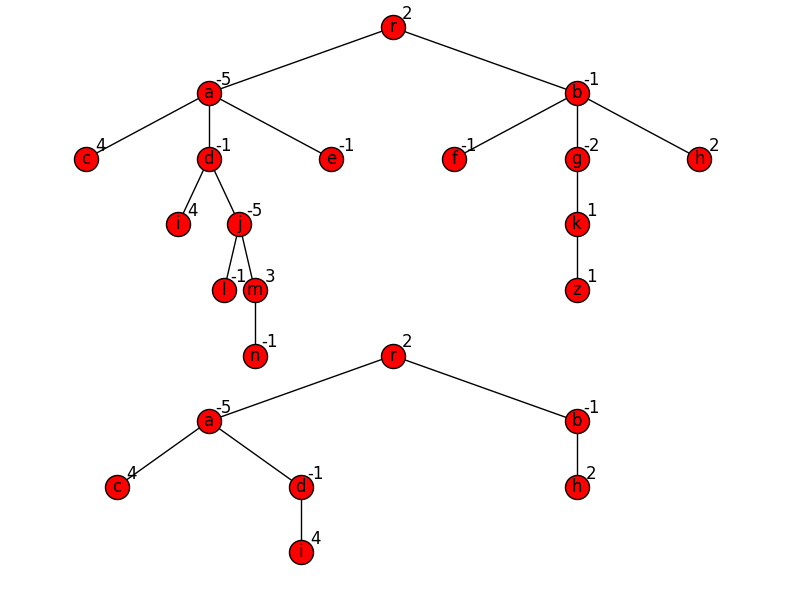
\includegraphics[width=\linewidth]{Arbre.png}
	\caption{Arbre de l'énoncé et son homologue maximisé}
\end{figure}
		\subsubsection{Fonctions et méthodes}
			
			
	\subsection{Complexité}
		\subsubsection{\texttt{get\_subSum}}
			\begin{figure}[h!]
				\centering
				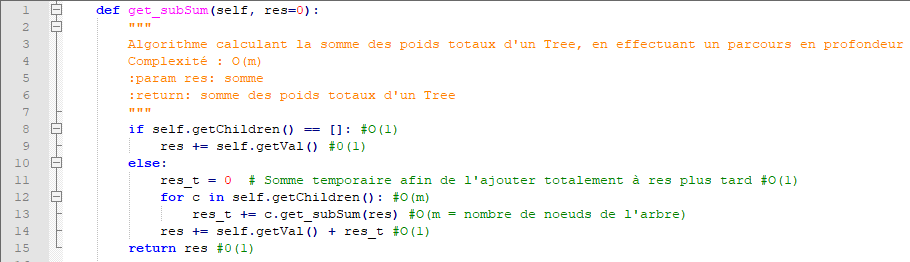
\includegraphics[width=\linewidth]{get_subSum.png}
				\caption{Fonction \texttt{get\_subSum}.}
			\end{figure}	
		
			Pour cette fonction, la ligne 8 et 9 sont en $O(1)$ car on appelle un accesseur et on effectue une somme. Même chose pour la ligne 14. En ce qui concerne la boucle à la ligne 12, la ligne 13 est en $O(m)$ ou $m$ est le nombre de nœuds dans l'arbre car on va l'appliquer sur tous les nœuds de l'arbre. Enfin, la boucle est en $O(m)$ où $m$ est le nombre de nœud de l'arbre complet. 
		\subsubsection{\texttt{max\_subtree}}
			\begin{figure}[h!]
				\centering
				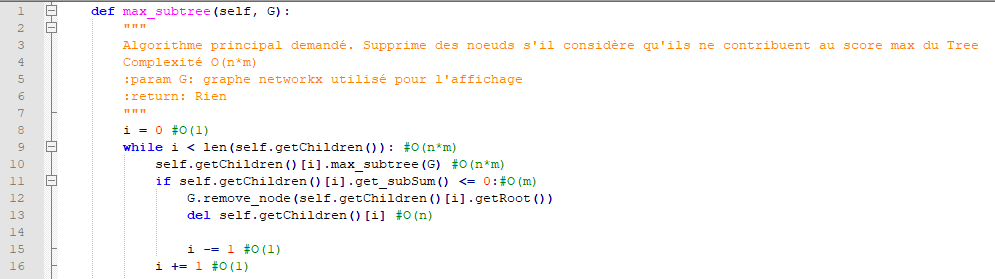
\includegraphics[width=\linewidth]{max_subtree.png}
				\caption{Fonction \texttt{max\_subtree}.}
			\end{figure}
			
			Cette fonction récursive a des instructions de $O(1)$ à la ligne 8, 15 et 16. À la ligne 13, nous avons cependant une complexité en $O(n)$ car la suppression d'un valeur dans une liste demande de réécrire toute la liste sans l'élément supprimé. Pour l'instruction \texttt{if} à la ligne 11, la complexité maximale est en $O(m)$ car c'est la complexité de la fonction \texttt{get\_subSum} calculée plus haut. En ce qui concerne celle de l'instruction de la ligne 10, nous avons déduit que le nombre d'appel de la fonction récursive est en $O(n*m)$ où $n$ est le nombre de fils.\\
			
			Nous pouvons enfin dire que la complexité maximale finale de la fonction est de $O(n*m)$. Néanmoins, nous pensons que la complexité est légèrement inférieure à cette valeur, car comme le montre la ligne 13, le nombre de fils varie, et donc par la même occasion le nombre de nœuds. Il ne faut pas non plus oublier que dans notre cas, les valeurs $m$ et $n$ sont assez petite. Elles varient entre 0 et 15, et 0 et 3 respectivement.
\section{Hypergraphe}
	\subsection{Implémentations}
		\subsubsection{Entrée et Sortie}
			En ce qui concerne l'entrée, nous avons opté pour une matrice d'incidence car il était plus simple de schématiser les arrêtes par une valeur booléenne. De plus, il était facile, via la librairie \texttt{Numpy} et sa méthode !!!random!!!, de générer des matrices aléatoires, ainsi que pour l'affichage qui sera décrit ci-dessous.
		\subsubsection{Affichage}
			Nous avons décidé d'afficher le graphe d'incidence, via la matrice d'incidence, le graphe dual, via une simple transposée de la matrice d'incidence et enfin le graphe primal du graphe dual. De cette façon, nous pouvons afficher plus facilement toutes les informations du graphe et de les comparer.\\

%afficher la matrice d'incidence ? 
%mettre des images de graphes
			
			Le terminal indiquera finalement si l'hypergraphe est un hypertree comme demandé. La matrice d'incidence est également affichée.
			

\begin{figure}[h!]
	\centering
	\begin{subfigure}[b]{0.45\linewidth}
		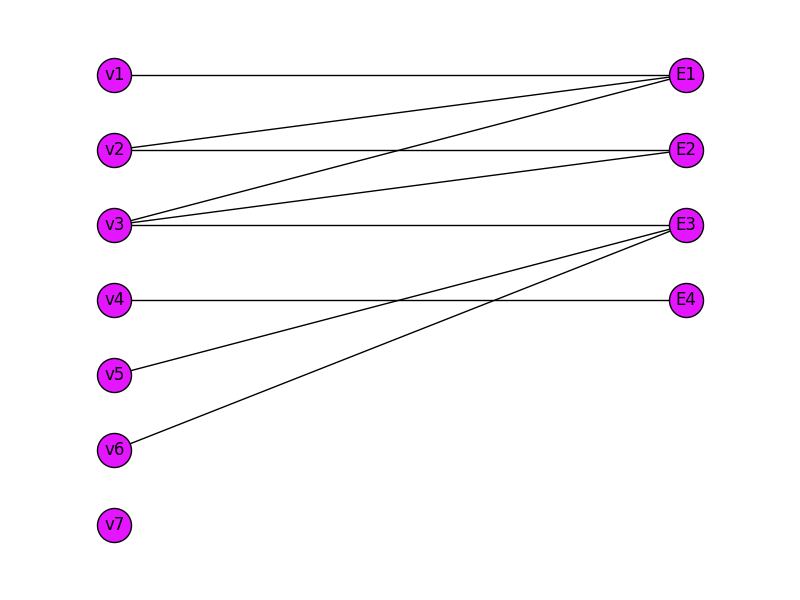
\includegraphics[width=\linewidth]{graphe_d'incidence.png}
  		\caption{Graphe d'incidence.}
	\end{subfigure}
	\begin{subfigure}[b]{0.45\linewidth}
		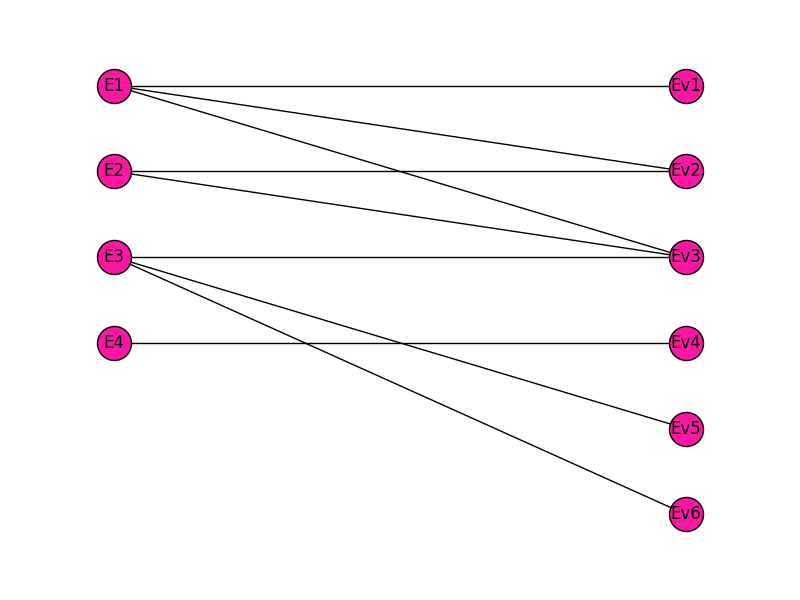
\includegraphics[width=\linewidth]{graphe_dual.png}
  		\caption{Graphe dual.}
  	\end{subfigure}
  	\begin{subfigure}[b]{0.5\linewidth}
		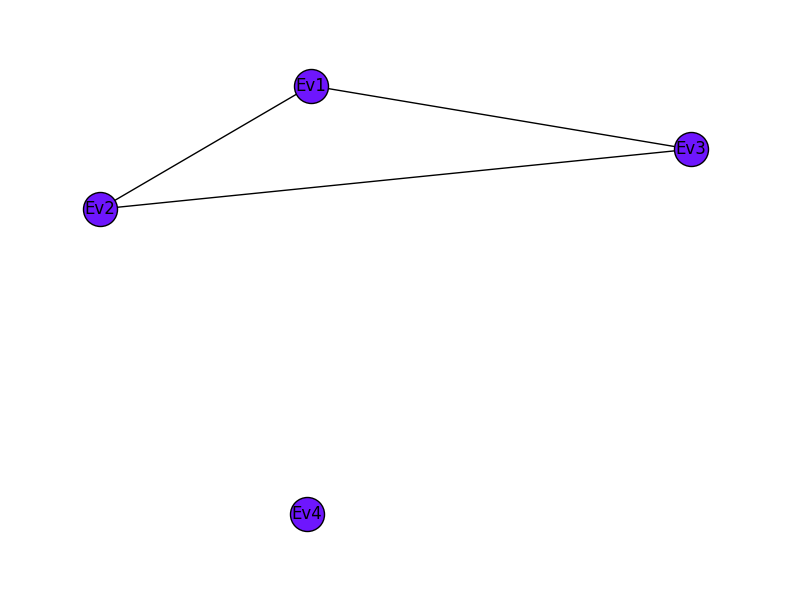
\includegraphics[width=\linewidth]{graphe_primal.png}
  		\caption{Graphe primal.}
  	\end{subfigure}
  	\caption{Affichage des différents graphes.}
\end{figure}

		\subsubsection{Fonctions et méthodes}
			En ce qui concerne le fonctionnement des méthodes et fonctions de notre implémentation, nous avons essayé de respecter un maximum la mécanique d'encapsulation, via l'utilisation de plusieurs accesseurs et mutateurs dans notre classe \texttt{Hypergraph}.\\
			
			Un objet de cette classe prend comme paramètre une matrice d'incidence, et via cette-dernière, va créer sa transposée. Avec ces 2 matrices, les graphes dual, primal et d'incidence seront créés.\\
			
			Pour pouvoir vérifier si un graphe est un hypertree ou non, nous devons tout d'abord vérifier s'il est cordal ou non. C'est ce que fait exactement la méthode \texttt{is\_chordal} de \texttt{networkx}. Elle prend en paramètre un graphe et retourne un booléen si oui ou non le graphe est cordal. 
			
			Si cette condition est vérifiée, on va analyser chaque clique maximale donnée par la méthode networkx \texttt{find\_cliques} dans la méthode \texttt{checkClique}. Cette dernière va avant tout créer un dictionnaire des hyperarêtes avec leurs sommets respectifs, pour ensuite comparer chaque clique maximale avec les sommets des hyperarrêtes. Si toutes les cliques sont présentes dans les hyperarêtes, alors la méthode renvoie \texttt{True}, et \texttt{False} sinon.
			

	\subsection{Complexité}	
			


\newpage
\tableofcontents

\end{document}
